Let 

\begin{align}
	\vec{A}= \myvec{-1\\2},  \vec{C}=\myvec{3\\2}.
\end{align}

The other two vertices can be obtained by using the following formula. 
\begin{align}
	\label{eq:square_points}
	\vec{B} = \frac{\norm{\vec{C}-\vec{A}}}{\sqrt{2}} \vec{P}\vec{e}_1+\vec{A}
	\\
	\vec{D} = \frac{\norm{\vec{C}-\vec{A}}}{\sqrt{2}} \vec{P}\vec{e}_2+\vec{A}
\end{align}
where 
\begin{align}
	\vec{P} = \myvec{\cos \brak{\theta-\frac{\pi}{4}} & -\sin  \brak{\theta-\frac{\pi}{4}} \\ \sin \brak{\theta-\frac{\pi}{4}} & \cos \brak{\theta-\frac{\pi}{4}}}
\end{align}
and 
\begin{align}
	\cos\theta = \frac{\brak{\vec{C}-\vec{A}}^{\top}\vec{e}_1}{\norm{\vec{C}-\vec{A}}\norm{\vec{e}_1}}
\end{align}
$\because $
\begin{align}
	\vec{C}-\vec{A} = \myvec{3\\2}- \myvec{-1\\2} =  \myvec{4\\0},
	\\
	\cos\theta  = 1 \implies \theta = 0
	\label{eq:square_points_theta}
\end{align}
Also, 
\begin{align}
	\vec{C}-\vec{A} &=4 
	\implies \frac{\norm{\vec{C}-\vec{A}}} {\sqrt{2}} = \frac{4}{\sqrt{2}}
	\label{eq:square_points_ratio}
\end{align}
Hence, using 
\eqref{eq:square_points},
\eqref{eq:square_points_theta} and 
\eqref{eq:square_points_ratio},
\begin{align}
	\vec{P}&= \frac{1}{\sqrt{2}}\myvec{1 & 1\\-1 & 1}, 
	\\
	\implies \vec{B} &= \frac{4}{2}\myvec{1 & 1\\-1 & 1} \myvec{1\\0}+ \myvec{-1\\2}
	\\
	&=\myvec{1\\0}
\end{align}

and 
\begin{align}
	\vec{D} &= \frac{4}{2}\myvec{1 & -1\\1 & 1} \myvec{0\\1}+ \myvec{-1\\2}
	\\
	&=\myvec{1\\4}
\end{align}
\begin{figure}[!ht]
	\centering
	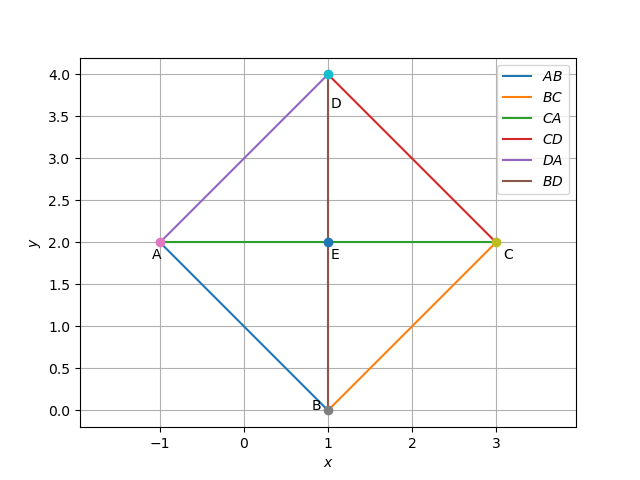
\includegraphics[width= \columnwidth]{solutions/1/6/quad.png}
\caption{Square ABCD}
\label{fig:2.2.7}
\end{figure}
See Fig. \ref{fig:2.2.7}.



